% --------------------------------------------------------------
\begin{frame}[fragile]
  \frametitle{Previous Work}
  \begin{itemize}
    \item Oak Ridge AHTR - unnecessary (Varma, Holcomb, et al.)
    \item COMSOL TH response analysis (Huff, Scarlat)
    \item Algebraic, 1-group LOFC neutronics analysis (Cisneros)
    \item Algebraic, 1-group RIA neutronics analysis (Greenspan, Fratoni)
  \end{itemize}

\end{frame}

% --------------------------------------------------------------
\begin{frame}[fragile]
  \frametitle{Pumping Power?}
  \begin{figure}[htbp!]
    \begin{center}
      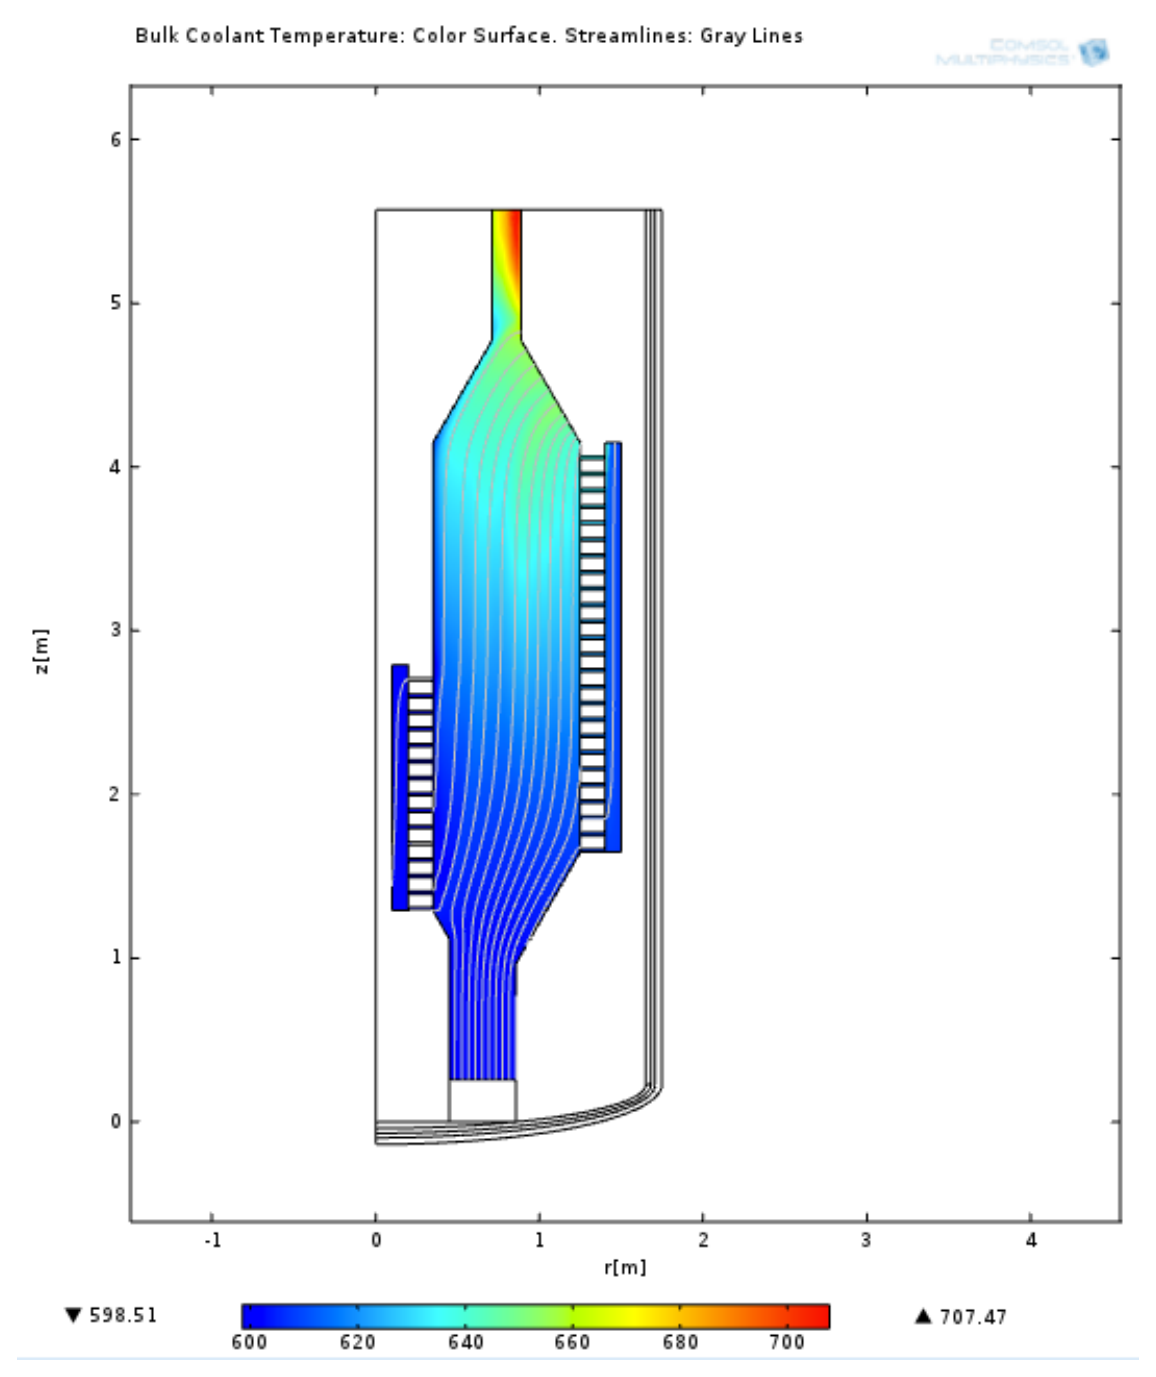
\includegraphics[width=0.8\textwidth]{./priorart/coolant_temps_100_deg_rise.eps}
    \end{center}
    \caption{For 100 degree temperature rise design point across the core.}
    \label{fig:200degrise}
  \end{figure}
\end{frame}

% --------------------------------------------------------------
\begin{frame}[fragile]
  \frametitle{Pumping Power?}

  \begin{figure}[htbp!]
    \begin{center}
      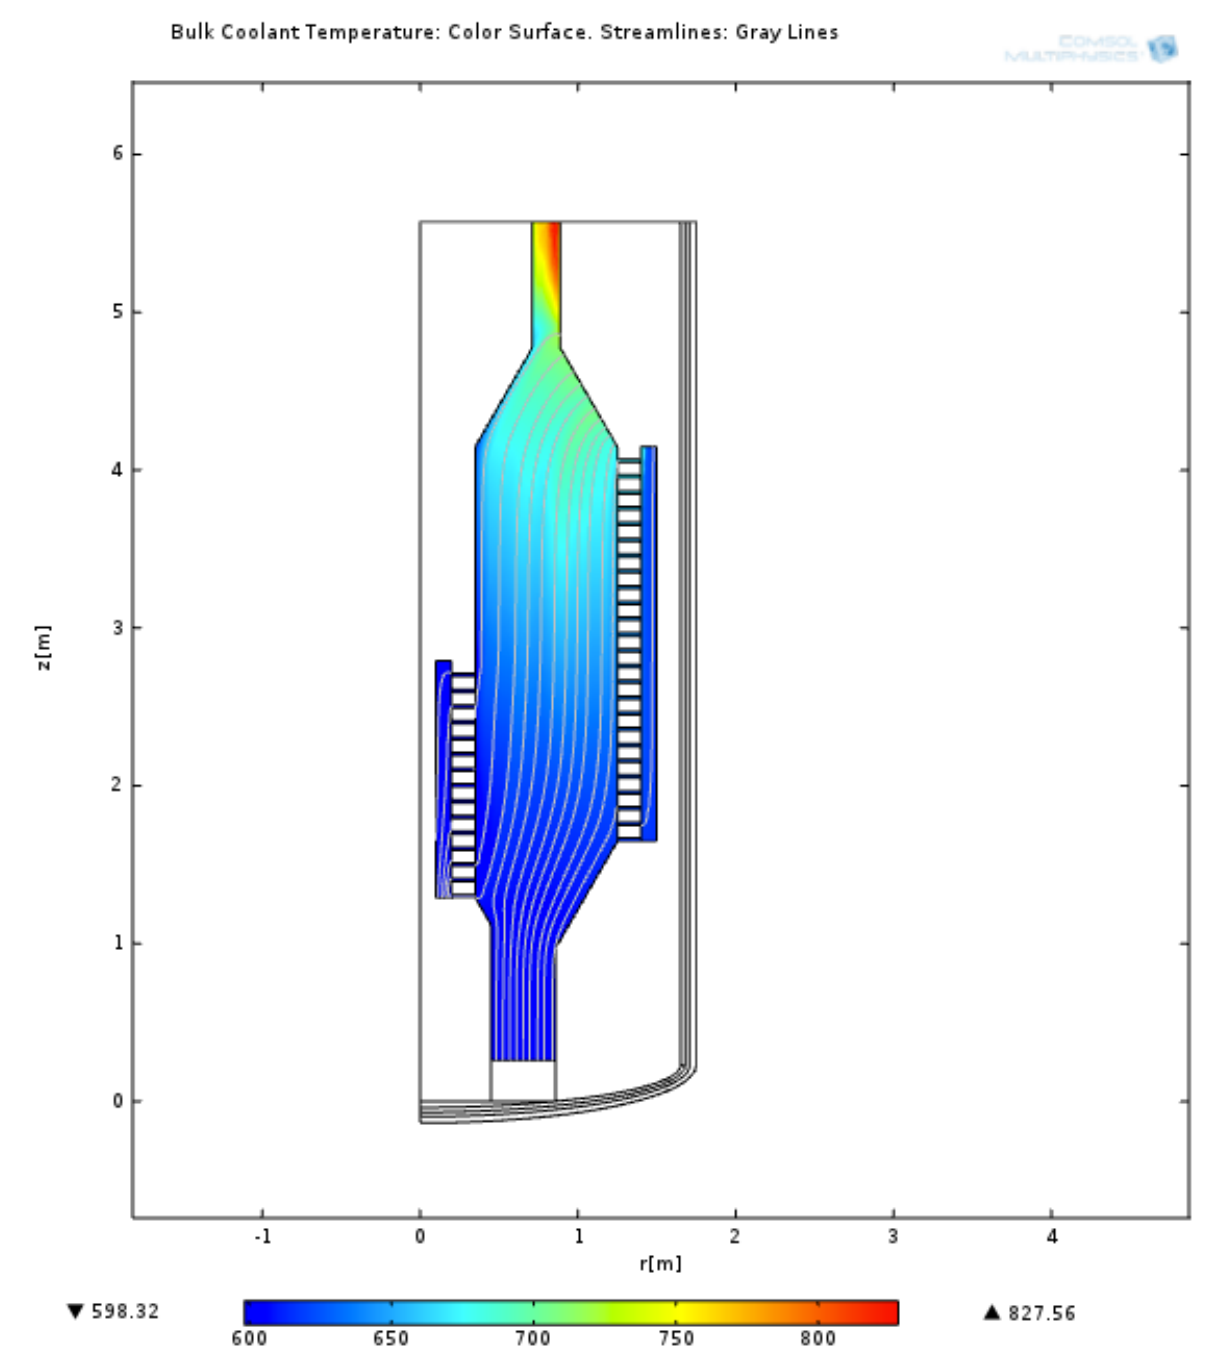
\includegraphics[width=0.8\textwidth]{./priorart/coolant_temps_200_deg_rise.eps}
    \end{center}
    \caption{For 200 degree temperature rise design point across the core.}
    \label{fig:200degrise}
  \end{figure}
\end{frame}

